Condor-G allows the user to treat the Grid as a local resource,
and the same command-line tools perform basic job management such as:
\begin{itemize}
\item Submit a job, indicating an executable, input and output files,
and arguments
\item Query a job's status
\item Cancel a job
\item Be informed when events happen,
such as normal job termination or errors
\item Obtain access to detailed logs that provide a complete history of a job
\end{itemize}

These are features that Condor has provided for many years.
Condor-G extends this to the grid,
providing resource management 
while still providing fault tolerance and exactly-once execution 
semantics. 


%%%%%%%%%%%%%%%%%%%%%%%%%%%%%%%%%%%%%%%%%%%%%%%%%%%%%%%%%%%%%%%%%%%%%%%%%%%
\subsection{\label{sec:Condor-G-Setup}Set Up of Condor-G}
%%%%%%%%%%%%%%%%%%%%%%%%%%%%%%%%%%%%%%%%%%%%%%%%%%%%%%%%%%%%%%%%%%%%%%%%%%%

%%%%%%%%%%%%%%%%%%%%%%%%%%%%%%%%%%%%%%%%%%%%%%%%%%%%%%%%%%%%%%%%%%%%%%%%%%%
\subsubsection{\label{sec:Condor-G-Install}Condor-G Installation}
%%%%%%%%%%%%%%%%%%%%%%%%%%%%%%%%%%%%%%%%%%%%%%%%%%%%%%%%%%%%%%%%%%%%%%%%%%%
\index{Condor-G!installation}
Condor-G is included in the standard Condor distribution.
Once Condor is obtained via download, installed, and configured,
(see
section~\ref{sec:install} on page~\pageref{sec:install})
there are two steps necessary before a globus universe job
can be submitted:

\begin{enumerate}

\item{Install Globus tools.}
Three ways are listed for obtaining the Globus tools:
   \begin{enumerate}
   \item{Globus}.
   From the web page at \URL{http://www.globus.org/}, follow links to the
   globus toolkit to get the resource management client bundle.
   \item{NMI}.
   From the web page at \URL{http://www.nsf-middleware.org/}, follow links
   to the NMI Release, and then to the Components, and finally to the
   Globus Toolkit. 
   \item{VDT}.
   From the web page at \URL{http://www.griphyn.org/vdt},
   follow the link to installing and setting up the Virtual Data Toolkit.
   \end{enumerate}

\item{Configure for Condor-G.}
If you installed Condor using the submit-only option, you will
need to add the following entries to your configuration file:
\footnotesize
\begin{verbatim}
GRIDMANAGER             = $(SBIN)/condor_gridmanager
GAHP                    = $(SBIN)/gahp_server
MAX_GRIDMANAGER_LOG     = 64000
GRIDMANAGER_DEBUG       = D_COMMAND
GRIDMANAGER_LOG         = $(LOG)/GridLogs/GridmanagerLog.$(USERNAME)
GLIDEIN_SERVER_URLS = \
  http://www.cs.wisc.edu/condor/glidein/binaries \
  gsiftp://gridftp.cs.wisc.edu/p/condor/public/binaries/glidein
\end{verbatim}
\normalsize

If Condor-G is installed as root, the file
set by the configuration variable
\Macro{GRIDMANAGER\_LOG} must have world-write permission.
All of the parent directories for this file must
also have world-execute permission.
The Gridmanager runs as the user who submitted the job,
so the Gridmanager may not be able to write to the ordinary 
\MacroUNI{log} directory.
%The example configuration file sets the log file to be 
%\begin{verbatim}
%GRIDMANAGER_LOG = $(LOG)/GridLogs/GridmanagerLog.$(USERNAME) 
%\end{verbatim}
Use of the definition of \MacroNI{GRIDMANAGER\_LOG}
shown above will likely require the creation of
the directory \verb@$(LOG)/GridLogs@.
Permissions on this directory should be set
by running \Prog{chmod} using the value 1777. 

Another option is to locate the Gridmanager log files
somewhere else, like so:
\begin{verbatim}
GRIDMANAGER_LOG  = /tmp/GridmanagerLog.$(USERNAME)
\end{verbatim}

If you make any changes to the configuration file while
Condor is running, you will need to issue a \Condor{reconfigure}
command.

Two additional configuration variables may be useful, 
in the case that a user submits many jobs at one time.
The configuration variable
\Macro{GRIDMANAGER\_MAX\_SUBMITTED\_JOBS\_PER\_RESOURCE}
limits the number of jobs
that a \Condor{gridmanager} daemon will submit to a resource.
It is useful for controlling the number of \Prog{jobmanager}
processes running on the front-end node of a cluster.
As an example,
consider the case where
\MacroNI{GRIDMANAGER\_MAX\_SUBMITTED\_JOBS\_PER\_RESOURCE}
is set to 100.
A user submits 1000 jobs to Condor-G, all intended to run
on the same resource.
Condor-G will start by only submitting 100 jobs to that resource.
As each submitted job completes,
Condor-G will submit another job from the remaining 900.
Without the throttle provided by this configuration variable,
Condor-G would submit all 1000 jobs together,
and the front-end node of the resource would be brought to its knees
by the corresponding
1000 Globus \Prog{jobmanager} processes.


A second useful configuration variable is
\Macro{GRIDMANAGER\_MAX\_PENDING\_SUBMITS\_PER\_RESOURCE},
the maximum number of jobs
that can be in the process of being submitted at any time (that is,
how many \Procedure{globus\_gram\_client\_job\_request} calls are pending).
It is useful for controlling the number of new
connections/processes created at a given time.
It exists because of a problem
when Condor-G tried to submit 100 jobs at one time,
and \Prog{inetd} on the remote host thought it was the
start of a denial-of-service attack (and therefore
disabled the gatekeeper service for a short period).

\MacroNI{GRIDMANAGER\_MAX\_SUBMITTED\_JOBS\_PER\_RESOURCE}
limits the total number of jobs that Condor-G will have submitted
to a remote resource at any given time.
\MacroNI{GRIDMANAGER\_MAX\_PENDING\_SUBMITS\_PER\_RESOURCE} limits
how fast Condor-G will submit jobs to a remote resource.
As an example, the configuration
\begin{verbatim}
GRIDMANAGER_MAX_SUBMITTED_JOBS_PER_RESOURCE=100
GRIDMANAGER_MAX_PENDING_SUBMITS_PER_RESOURCE=20
\end{verbatim}
will have Condor-G submit jobs in sets of 20 until a total of 100 have
been submitted.

See section~\ref{sec:Configuring-Condor} on
page~\pageref{sec:Configuring-Condor} for
more information about configuration file entries.
See section~\ref{sec:Gridmanager-Config-File-Entries} on
page~\pageref{sec:Gridmanager-Config-File-Entries} for information
about  configuration file entries specific to the Condor-G
gridmanager.

\end{enumerate}

%%%%%%%%%%%%%%%%%%%%%%%%%%%%%%%%%%%%%%%%%%%%%%%%%%%%%%%
\subsubsection{\label{sec:Condor-G-Credentials}Configuration for Credential Management}
%%%%%%%%%%%%%%%%%%%%%%%%%%%%%%%%%%%%%%%%%%%%%%%%%%%%%%%

%(Reword this section to talk more about credential management and less
%about specific config values. Also, probably move it out of the setup
%section.)

Condor-G periodically checks for an updated proxy at
\index{Condor-G!proxy}
\index{proxy}
an interval given by the configuration variable
\AdAttr{GRIDMANAGER\_CHECKPROXY\_INTERVAL}.
The value is defined in terms of seconds.
For example, if you create a 12-hour proxy, and then
6 hours later re-run \Prog{grid-proxy-init},
Condor-G will check the proxy within
this time interval, and use the new proxy it finds there.
The default interval is 10 minutes.

Condor-G also knows when the proxy of each job will expire,
and if the proxy is not refreshed before
\AdAttr{GRIDMANAGER\_MINIMUM\_PROXY\_TIME}
seconds before the proxy expires,
the Condor-G grid manager daemon exits.
Since the grid manager daemon keeps track of all jobs
associated with a proxy, its tasks
(such as authentication, file transfer, job log maintenance)
will not occur.
So, if
\AdAttr{GRIDMANAGER\_MINIMUM\_PROXY\_TIME}
is 180, and the proxy is 3 minutes away from
expiring, Condor-G will attempt to safely shut down,
instead of simply losing
contact with the remote job because Condor-G is unable to
authenticate the remote job.
The default setting is 3 minutes (180 seconds).

%%%%%%%%%%%%%%%%%%%%%%%%%%%%%%%%%%%%%%%%%%%%%%%%%%%%%%%%%%%%%%%%%%%%%%%%%%%
\subsection{\label{sec:Grid-using}Using the Grid Universe}
%%%%%%%%%%%%%%%%%%%%%%%%%%%%%%%%%%%%%%%%%%%%%%%%%%%%%%%%%%%%%%%%%%%%%%%%%%%
\index{grid universe}
\index{universe!grid}

%%%%%%%%%%%%%%%%%%%%%%%%%%%%%%%%%%%%%%%%%%%%%%%%%%%%%%%%%%%%%%%%%%%%%%%%%%%
\subsubsection{\label{sec:Globus-Protocols}Globus and Its Protocols}
%%%%%%%%%%%%%%%%%%%%%%%%%%%%%%%%%%%%%%%%%%%%%%%%%%%%%%%%%%%%%%%%%%%%%%%%%%%
The Globus software provides a well-defined set of protocols
that allow authentication, data transfer, and remote job submission.
Authentication is a mechanism by which an identity is verified.
Given proper authentication, authorization to use a resource
is required.
Authorization is a policy that determines who is allowed to do what. 

Starting with Condor Version 6.7.0, the \AdAttr{grid} universe
replaces the \AdAttr{globus} universe.
Further specification of a \AdAttr{grid} universe job is done
within the \AdAttr{grid\_type} command in a submit description file.
Older submit description files specifying the \AdAttr{globus} 
universe will become \AdAttr{grid} universe jobs using the
Globus \AdAttr{gt2} protocol.

It may appear that Condor-G is a simple replacement
for the Globus toolkit's \Prog{globusrun} command.
However, Condor-G does much more.
It allows the submission of many jobs at once
along with the monitoring of those jobs with a convenient interface.
There is notification when jobs complete or fail
and maintenance Globus credentials
that may expire while a job is running.
On top of this, Condor-G is a fault-tolerant system;
if your machine crashes,
you can still perform all of these functions when your machine returns to life.


Condor uses the following Globus protocols.
These protocols allow Condor to utilize grid machines for
the execution of jobs.
\begin{description}
\item[GSI]
\index{GSI (Grid Security Infrastructure)}
The Globus Toolkit's Grid Security Infrastructure (GSI) provides essential
\index{Condor-G!GSI}
building blocks for other Grid protocols and Condor-G.
This authentication and authorization system
makes it possible to authenticate a user just once,
using public key infrastructure (PKI) mechanisms to verify
a user-supplied grid credential.
GSI then handles the mapping of the grid credential to the
diverse local credentials and authentication/authorization mechanisms that
apply at each site. 
\item[GRAM]
The Grid Resource Allocation and Management (GRAM) protocol supports remote
\index{Condor-G!GRAM}
\index{GRAM (Grid Resource Allocation and Management)}
submission of a computational request (for example, to run program P)
to a remote computational resource,
and it supports subsequent monitoring and control of the resulting
computation. 
GRAM is the Globus protocol that Condor-G uses to talk to remote Globus
  jobmanagers.
\item[GASS]
The Globus Toolkit's Global Access to Secondary Storage (GASS) service provides
\index{Condor-G!GASS}
\index{GASS (Global Access to Secondary Storage)}
mechanisms for transferring data to and from a remote HTTP, FTP, or GASS server. 
Condor-G uses GASS to transfer the executable, 
\File{stdin}, 
\File{stdout}, and 
\File{stderr}
between the machine where a job is submitted and the remote resource.
\item[RSL]
RSL is the language GRAM accepts to specify job information.
\end{description}


\begin{figure}[hbt]
\centering
\includegraphics{grids/gfig1.eps}
\caption{\label{fig:condorg}Remote Execution by Condor-G on Globus-managed resources}
\end{figure}

Figure~\ref{fig:condorg} shows how Condor-G interacts with Globus protocols.
Condor-G contains a GASS server, used to transfer the executable,
\File{stdin}, \File{stdout}, and \File{stderr} to and from
the remote job execution site.
Condor-G uses the GRAM protocol to contact the remote Globus Gatekeeper
and request that a new job manager be started.
GRAM is also used to monitor the job's progress.
Condor-G detects and intelligently handles cases
such as if the remote Globus resource crashes.

%%%%%%%%%%%%%%%%%%%%%%%%%%%%%%%%%%%%%%%%%%%%%%%%%%%%%%%%%%%%%%%%%%%%%%%%%%%
\subsubsection{\label{sec:Using-gt2}Grid Universe Jobs with grid\_type gt2}
%%%%%%%%%%%%%%%%%%%%%%%%%%%%%%%%%%%%%%%%%%%%%%%%%%%%%%%%%%%%%%%%%%%%%%%%%%%

\index{universe!globus}
\index{universe!grid, grid\_type gt2}
This section contains what users need to know to 
run and manage jobs under the \AdAttr{grid} universe, using the Globus \AdAttr{gt2} protocol.
Older submit description files specifying a \AdAttr{globus} universe job
will default to this.

\index{Condor-G!job submission}
\index{Condor-G!proxy}
\index{proxy}
Under Condor, successful job submission to the \AdAttr{grid} universe with \AdAttr{gt2}
requires credentials.
\index{Condor-G!X.509 certificate}
An X.509 certificate is used to create a proxy,
and an account, authorization, or allocation to use a grid resource
is required.
For more information on proxies and certificates,
please consult the Alliance PKI pages at 

\URL{http://archive.ncsa.uiuc.edu/SCD/Alliance/GridSecurity/}

Before submitting a job to Condor under the \AdAttr{grid} universe,
make sure you have your Grid 
credentials and have used \Prog{grid-proxy-init} to create a proxy.

A job is submitted for execution to Condor using the
\Condor{submit} command.
\index{Condor commands!condor\_submit}
\Condor{submit} takes as an argument
the name of a file called a submit description file.
\index{submit description file!grid universe}
The following sample submit description file runs a job on
the Origin2000 at NCSA.

\begin{verbatim}
executable = test
globusscheduler = modi4.ncsa.uiuc.edu/jobmanager
universe = grid
grid_type = gt2
output = test.out
log = test.log
queue
\end{verbatim} 

The 
\AdAttr{executable}
for this example is
transferred from the local machine to the remote machine.
By default, Condor transfers the executable, as well as any
files specified by the \AdAttr{input} command.
Note that this executable must be compiled for the correct
intended platform.

The \AdAttr{globusscheduler} command is dependent on the
scheduling software available on remote resource.
This required command will change based on the Grid resource
intended for execution of the job.
A jobmanager is the Globus service that is spawned at a remote site to
submit, keep track of, and manage Grid I/O for jobs running on the local
batch system there.
There is a specific jobmanager for each type of
batch system supported by Globus (examples are Condor, LSF, and PBS).

All Condor-G jobs 
submitted to the \AdAttr{globus} universe
are identical to those submitted to the \AdAttr{grid} universe,
with \AdAttr{grid\_type} set to \AdAttr{gt2}.

No input file is specified for this example job.
Any output (file specified by the \AdAttr{output})
or error (file specified by the \AdAttr{error})
is transferred 
from the remote machine to the local machine as it is produced.
This implies that these files may be incomplete in the case
where the executable does not finish running on the remote resource.
The ability to transfer standard output and standard error as
they are produced may be disabled by adding to the submit
description file:
\begin{verbatim}
stream_output = False
stream_error  = False
\end{verbatim}
As a result, standard output and standard error will be transferred
only after the job completes.

The job log file is maintained on the submit machine.

To submit this job to Condor-G for execution on the
remote machine, use
\begin{verbatim}
condor_submit test.submit
\end{verbatim}
where \File{test.submit} is the name of the submit description file.

Example output from 
\Condor{q} for this submission looks like:
\footnotesize
\begin{verbatim}
% condor_q


-- Submitter: wireless48.cs.wisc.edu : <128.105.48.148:33012> : wireless48.cs.wi

 ID      OWNER         SUBMITTED     RUN_TIME ST PRI SIZE CMD
   7.0   epaulson     3/26 14:08   0+00:00:00 I  0   0.0  test

1 jobs; 1 idle, 0 running, 0 held
\end{verbatim}
\normalsize

After a short time, the Globus resource accepts the job.
Again running \Condor{q} will now result in

\footnotesize
\begin{verbatim}
% condor_q


-- Submitter: wireless48.cs.wisc.edu : <128.105.48.148:33012> : wireless48.cs.wi

 ID      OWNER         SUBMITTED     RUN_TIME ST PRI SIZE CMD
   7.0   epaulson     3/26 14:08   0+00:01:15 R  0   0.0  test

1 jobs; 0 idle, 1 running, 0 held
\end{verbatim}
\normalsize

Then, very shortly after that, the queue will be empty again,
because the job has finished:

\footnotesize
\begin{verbatim}
% condor_q


-- Submitter: wireless48.cs.wisc.edu : <128.105.48.148:33012> : wireless48.cs.wi

 ID      OWNER            SUBMITTED     RUN_TIME ST PRI SIZE CMD

0 jobs; 0 idle, 0 running, 0 held
\end{verbatim}
\normalsize


A second example of a submit description file runs the Unix \Prog{ls}
program on a different Globus resource.

\footnotesize
\begin{verbatim}
executable = /bin/ls
Transfer_Executable = false
globusscheduler = vulture.cs.wisc.edu/jobmanager
universe = grid
grid_type = gt2
output = ls-test.out
log = ls-test.log
queue
\end{verbatim} 
\normalsize

In this example, the executable (the binary) has been pre-staged.
The executable is on the remote machine, and it is not to
be transferred before execution.
Note that the required 
\AdAttr{globusscheduler} and \AdAttr{universe}
commands are present.
The command
\begin{verbatim}
Transfer_Executable = false
\end{verbatim}
within the submit description file identifies the executable
as being pre-staged.
In this case, the 
\AdAttr{executable}
command gives the path to the executable on the remote machine.

A third example submits a Perl script to be run as a submitted
Condor job.
The Perl script both lists and sets
environment variables for a job.
Save the following Perl script with the name \File{env-test.pl},
to be used as a Condor job executable.

\begin{verbatim}
#!/usr/bin/env perl

foreach $key (sort keys(%ENV))
{
   print "$key = $ENV{$key}\n"
}

exit 0;
\end{verbatim}

Run the Unix command
\begin{verbatim}
chmod 755 env-test.pl
\end{verbatim}
to make the Perl script executable.

Now create the following submit description file
(Replace \File{biron.cs.wisc.edu/jobmanager} with a resource
you are authorized to use.):

\footnotesize
\begin{verbatim}
executable = env-test.pl
globusscheduler = biron.cs.wisc.edu/jobmanager
universe = grid
grid_type = gt2
environment = foo=bar; zot=qux
output = env-test.out
log = env-test.log
queue
\end{verbatim}
\normalsize

When the job has completed, the output file \File{env-test.out}
should contain something like this:

\footnotesize
\begin{verbatim}
GLOBUS_GRAM_JOB_CONTACT = https://biron.cs.wisc.edu:36213/30905/1020633947/
GLOBUS_GRAM_MYJOB_CONTACT = URLx-nexus://biron.cs.wisc.edu:36214
GLOBUS_LOCATION = /usr/local/globus
GLOBUS_REMOTE_IO_URL = /home/epaulson/.globus/.gass_cache/globus_gass_cache_1020633948
HOME = /home/epaulson
LANG = en_US
LOGNAME = epaulson
X509_USER_PROXY = /home/epaulson/.globus/.gass_cache/globus_gass_cache_1020633951
foo = bar
zot = qux
\end{verbatim}
\normalsize


Of particular interest is the GLOBUS\_REMOTE\_IO\_URL environment variable.
Condor-G automatically starts up a GASS remote I/O
server on the submitting machine.
Because of the potential for either side of the connection to fail,
the URL for the server cannot be passed directly to the job.
Instead, it is put into a file, and the GLOBUS\_REMOTE\_IO\_URL
environment variable points to this file. 
Remote jobs can read this file and use the URL it contains
to access the remote GASS server running inside Condor-G.
If the location
of the GASS server changes (for example, if Condor-G restarts),
Condor-G will contact the Globus gatekeeper and update this file on
the machine where the job is running.
It is therefore important that all accesses to
the remote GASS server check this file for the latest location.

The following example is a Perl script that uses the GASS server in Condor-G
to copy input files to the execute machine.
In this example, the remote job
counts the number of lines in a file.

\footnotesize
\begin{verbatim}
#!/usr/bin/env perl
use FileHandle;
use Cwd;

STDOUT->autoflush();
$gassUrl = `cat $ENV{GLOBUS_REMOTE_IO_URL}`;
chomp $gassUrl;

$ENV{LD_LIBRARY_PATH} = $ENV{GLOBUS_LOCATION}. "/lib";
$urlCopy = $ENV{GLOBUS_LOCATION}."/bin/globus-url-copy";

# globus-url-copy needs a full pathname
$pwd = getcwd();
print "$urlCopy $gassUrl/etc/hosts file://$pwd/temporary.hosts\n\n";
`$urlCopy $gassUrl/etc/hosts file://$pwd/temporary.hosts`;

open(file, "temporary.hosts");
while(<file>) {
print $_;
}

exit 0;
\end{verbatim}
\normalsize

The submit description file used to submit the Perl script as
a Condor job appears as:

\footnotesize
\begin{verbatim}
executable = gass-example.pl
globusscheduler = biron.cs.wisc.edu/jobmanager
universe = grid
grid_type = gt2
output = gass.out
log = gass.log
queue
\end{verbatim}
\normalsize

There are two optional submit description file commands
of note:
\AdAttr{x509userproxy} and
\AdAttr{globusrsl}.
The \AdAttr{x509userproxy} command specifies the path to
an X.509 proxy.
The command is of the form:
\begin{verbatim}
x509userproxy = /path/to/proxy
\end{verbatim}
If this optional command is not present in the submit description file,
then Condor-G checks the value of the environment variable
\Env{X509\_USER\_PROXY} for the location of the proxy.
If this environment variable is not present, then Condor-G
looks for the proxy in the file
\File{/tmp/x509up\_u0000},
where the trailing zeros in this file name are
replaced with the Unix user id.

The \AdAttr{globusrsl} command is used to add additional
attribute settings to a job's RSL string.
The format of the \AdAttr{globusrsl} command is
\begin{verbatim}
globusrsl = (name=value)(name=value)
\end{verbatim}
Here is an example of this command from a submit description file:
\begin{verbatim}
globusrsl = (project=Test_Project)
\end{verbatim}
This example's attribute name for the additional RSL is
\AdAttr{project}, and the value assigned is \AdAttr{Test\_Project}.

%%%%%%%%%%%%%%%%%%%%%%%%%%%%%%%%%%%%%%%%%%%%%%%%%%%%%%%%%%%%%%%%%%%%%%%%%%%
\subsubsection{\label{sec:Using-gt3}Grid Universe Jobs with grid\_type gt3}
%%%%%%%%%%%%%%%%%%%%%%%%%%%%%%%%%%%%%%%%%%%%%%%%%%%%%%%%%%%%%%%%%%%%%%%%%%%
\index{universe!grid, grid\_type gt3}

Condor-G version 6.7.1 allows the user to submit jobs
to Globus Toolkit 3.2 (gt3) gatekeepers,
in a manner similar to the submission of
jobs to Globus 2.x gatekeepers.
Condor-G version 6.7.1 supports submission of jobs to gatekeepers
running web services from GT 3.2.
Please note that this is \emph{not} compatible with GT 3.0.

See
\URL{http://www-unix.globus.org/toolkit/docs/3.0/index.html}
for more information about Globus Toolkit 3.0.

In order to submit \AdAttr{grid\_type} \AdAttr{GT3} jobs,
the following items must be defined in the user's
submit description file:
\footnotesize
\begin{verbatim}
universe = grid
grid_type = gt3
Executable = /bin/foo
Globusscheduler = http://198.51.254.40:8080/ogsa/services/base/gram/ForkMa
nagedJobFactoryService
\end{verbatim}
\normalsize

as well as other useful parameters such as
\AdAttr{log} and \AdAttr{transfer\_executable}.
The value for \AdAttr{globusscheduler} is placed on two lines for
formatting purposes, but will all be on a single line within
a submit description file.
Its value is the URL of the appropriate GT3 job factory service.
It is the same, for example,
as the URL provided to the \Prog{managed-job-globusrun} tool in GT3.

The user is not required to have any GT3 components installed on the
submitting machine.
Condor installs all the necessary GT3 client framework under 
\File{\MacroUNI{LIB}/lib/gt3}.
The user is, however, required to
have Java 1.4 or higher installed on the submitting machine,
and it must be referenced by the 
\Macro{JAVA} configuration macro.

In order to debug submission of GT3 jobs,
the user may utilize the optional configuration variable
\Macro{GT3\_GAHP\_LOG} to point at a
file where the debug information from GT3 GAHP (the component that
interfaces between Condor and GT3) will be sent.


%%%%%%%%%%%%%%%%%%%%%%%%%%%%%%%%%%%%%%%%%%%%%%%%%%%%%%%%%%%%%%%%%%%%%%%%%%%
\subsubsection{\label{sec:CondorG-Submit-Args}Arguments to a Grid Universe Job}
%%%%%%%%%%%%%%%%%%%%%%%%%%%%%%%%%%%%%%%%%%%%%%%%%%%%%%%%%%%%%%%%%%%%%%%%%%%
\index{Condor-G!job arguments}

Condor requires space characters to delimit the arguments
in an submit description file such as
\begin{verbatim}
arguments = 13 argument2 argument3
\end{verbatim}
This example results in the 3 arguments:
\begin{verbatim}
argv[1] = 13
argv[2] = argument2
argv[3] = argument3
\end{verbatim}

With Condor-G, arguments are passed through using RSL.
Therefore, arguments are parsed in a way that allows space characters
to be delimiters or to be parts of arguments.
The single quote character delimits some or all arguments such that
\begin{verbatim}
arguments = '%s' 'argument with spaces' '+%d'
\end{verbatim}
results in
\begin{verbatim}
argv[1] = %s
argv[2] = argument with spaces
argv[3] = +%d
\end{verbatim}

Should the arguments themselves contain the single quote character,
an escaped double quote character may be used.
The example
% % what it is supposed to appear as:
% % arguments = \"don't\" \"mess with\" \"quoting rules\"
\footnotesize
\begin{verbatim}
arguments = \"don't\" \"mess with\" \"quoting rules\"
\end{verbatim}
\normalsize
results in 
\begin{verbatim}
argv[1] = don't
argv[2] = mess with
argv[3] = quoting rules
\end{verbatim}

And, if the job arguments have both single and double quotes,
the appearance of the quote character twice in a
row is converted to a single instance of the character and the literal
continues until the next solo quote character.
For example
\begin{verbatim}
arguments = 'don''t yell \"blah!\"' '+%s'
\end{verbatim}
results in
\begin{verbatim}
argv[1] = don't yell "blah!"
argv[2] = +%s
\end{verbatim}


%%%%%%%%%%%%%%%%%%%%%%%%%%%%%%%%%%%%%%%%%%%%%%%%%%%%%%%%%%%%%%%%%%%%%%%%%%%
\subsubsection{\label{sec:My-Proxy}Credential Management with \Prog{MyProxy}}
%%%%%%%%%%%%%%%%%%%%%%%%%%%%%%%%%%%%%%%%%%%%%%%%%%%%%%%%%%%%%%%%%%%%%%%%%%%
\index{proxy!renewal with \Prog{MyProxy}}
Condor-G can use \Prog{MyProxy}
software to automatically renew GSI proxies for
\AdAttr{globus} or
\AdAttr{grid}
universe jobs with a
\AdAttr{grid\_type} of either
\AdStr{gt2}
or
\AdStr{gt3}.

\Prog{MyProxy} is a software component developed at
NCSA and used widely throughout the grid community.
For more information see:
\URL{http://myproxy.ncsa.uiuc.edu/}

Difficulties with proxies occur
when jobs are long running or a
great number of jobs submitted,
in which case some jobs may not be started
or completed before the proxy expires.
One proposed solution to these difficulties is to generate
longer-lived proxies.
This, however, presents a greater security problem.
Remember that a GSI proxy is sent to the remote Globus resource.
If a proxy falls into the hands of a malicious user at the remote site,
the malicious user can impersonate the proxy owner
for the duration of the proxy's lifetime.
The longer the proxy's lifetime,
the more time a malicious user has to misuse the owner's credentials.
To minimize the malicious user's window of opportunity,
it is recommended that proxies have a short lifetime
(on the order of several hours).

The \Prog{MyProxy} software generates proxies using credentials
(a user certificate or a long-lived proxy) located on a secure
\Prog{MyProxy} server.
Condor-G can talk to a MyProxy server,
renewing a proxy whenever it is about to expire.
Another advantage that this presents is it relieves the user
from having to store a GSI user certificate and private key
on the machine where jobs are submitted.
This may be particularly important if a shared Condor-G
submit machine is used by several users.

In the a typical case, the following steps occur:

\begin{enumerate}
\item{User creates a long-lived credential}
on a secure \Prog{MyProxy} server, using the
\Prog{myproxy-init} command.
Each organization generally has their own \Prog{MyProxy} server.

\item{User creates a short-lived proxy}
on a local submit machine,
using
\Prog{grid-proxy-init} or \Prog{myproxy-get-delegation}.

\item{User submits}
a Condor-G job,
specifying in the submit file:
\begin{description}
\item{\Prog{MyProxy} server name (host:port)}
\item{\Prog{MyProxy} credential name (optional)}
\item{\Prog{MyProxy} password}
\end{description}

\item{At the short-lived proxy expiration}
Condor-G talks to
the \Prog{MyProxy} server to refresh the proxy.

\end{enumerate}

A typical submit description file that uses \Prog{MyProxy} will
contain commands of the form:
\footnotesize
\begin{verbatim}
executable      = /usr/bin/my-executable
universe        = grid
grid_type       = "gt3"
globusscheduler = condor-unsup-7
MyProxyHost     = beak.cs.wisc.edu:7512
MyProxyServerDN = /O=doesciencegrid.org/OU=People/CN=Jane Doe 25900
MyProxyPassword = password
MyProxyCredentialName = my_executable_run
queue
\end{verbatim}
\normalsize

Condor-G keeps track of the password to the \Prog{MyProxy} server
for credential renewal.
Although Condor-G tries to keep the password encrypted and secure,
it is still possible (although highly unlikely) for the password
to be intercepted from the Condor-G machine
(more precisely, from the machine that the
\Condor{schedd} daemon that manages the grid universe jobs runs on,
which may be distinct from the machine from where jobs are submitted).
The following safeguard practices are recommended.

\begin{enumerate}

\item{Provide time limits}
for credentials on the \Prog{MyProxy} server.
The default is one week, but you may want to make it shorter.
%(See --cred_lifetime option to myproxy-init).

\item{Create several different \Prog{MyProxy} credentials},
maybe as many as one for each submitted job.
Each credential has a unique name,
which is identified with the
\Attr{MyProxyCredentialName} command in the submit description file.

\item{Use the following options}
when initializing the credential on the \Prog{MyProxy} server:

\footnotesize
\begin{verbatim}
myproxy-init -s <host> -x -r <cert subject> -k <cred name>
\end{verbatim}
\normalsize

The option \OptArg{-x -r}{<cert subject>}
essentially tells the \Prog{MyProxy} server to require two forms
of authentication:
  \begin{enumerate}
  \item{a password (initially set with \Prog{myproxy-init})}
  \item{an existing proxy (the proxy to be renewed)}
  \end{enumerate}

\item{Use the \Opt{-p} option to \Condor{submit}}
to avoid using the password in the submit description file.
The submit command appears as
\footnotesize
\begin{verbatim}
condor_submit -p mypassword /home/user/myjob.submit
\end{verbatim}
\normalsize

\end{enumerate}

Currently, Condor-G calls the
\Prog{myproxy-get-delegation} command-line tool,
passing it the necessary arguments.
The location of the
\Prog{myproxy-get-delegation} executable is determined by the
configuration variable
\Macro{MYPROXY\_GET\_DELEGATION} in the configuration file
on the Condor-G machine.
This variable is read by the \Condor{gridmanager}.
If
\Prog{myproxy-get-delegation}
is a dynamically-linked executable
(verify this with \Code{ldd myproxy-get-delegation}),
point
\MacroNI{MYPROXY\_GET\_DELEGATION}
to a wrapper shell script that sets
\MacroNI{LD\_LIBRARY\_PATH} to the correct \Prog{MyProxy}
library or Globus library directory and then
calls \Prog{myproxy-get-delegation}.
Here is an example of such a wrapper script:

\footnotesize
\begin{verbatim}
#!/bin/sh
export LD_LIBRARY_PATH=/opt/myglobus/lib
exec /opt/myglobus/bin/myproxy-get-delegation $@
\end{verbatim}
\normalsize


%%%%%%%%%%%%%%%%%%%%%%%%%%%%%%%%%%%%%%%%%%%%%%%%%%%%%%%%%%%%%%%%%%%%%%%%%%%
\subsubsection{Removing Condor-G jobs}
%%%%%%%%%%%%%%%%%%%%%%%%%%%%%%%%%%%%%%%%%%%%%%%%%%%%%%%%%%%%%%%%%%%%%%%%%%%

When you remove a job with \Condor{rm}, you may find that the job
enters the ``X'' state for a very long time. This is normal: Condor-G
is attempting to communicate with the remote Globus resource and
ensure that the job has been properly cleaned up. If it takes too long
or (in rare circumstances) is never removed, you can force the job to
leave the job queue by using the -forcex option to \Condor{rm}. This
will forcibly remove jobs that are in the X state without attempting
to finish any cleanup at the remote resource.


%%%%%%%%%%%%%%%%%%%%%%%%%%%%%%%%%%%%%%%%%%%%%%%%%%%%%%%%%%%%%%%%%%%%%%%%%%%
\subsubsection{\label{sec:Condor-G-Limits}Limitations of Condor-G}
%%%%%%%%%%%%%%%%%%%%%%%%%%%%%%%%%%%%%%%%%%%%%%%%%%%%%%%%%%%%%%%%%%%%%%%%%%%
% This subsubsection used to reside in the file limitations.tex.
\index{Condor-G!limitations}
Submitting jobs to run under the globus universe has not yet
been perfected.
The following is a list of known limitations:

\begin{enumerate}
\item{No checkpoints.}
\item{No job exit codes.}
Job exit codes are not available.
\item{Limited platform availability.}
Condor-G is only available on Linux, Solaris,
Digital UNIX, and IRIX.
HP-UX support will hopefully be available later.
\end{enumerate}
